\section{Gradient-based Adversarial Attacks}

% \begin{frame}{Neural Network Training}
%     What does it mean to train a Neural Network classifier?
%     \vfill
    
%     \note{We have the input, then}

%     \begin{minipage}{0.2\linewidth}
%         \centering
%         
\includegraphics[width=\linewidth]{assets/input_cat.png}\\
%         Input image
%     \end{minipage}\hfill
%     \note{We give it to a neural network}
%     %
%     \begin{minipage}{0.4\linewidth}
%         \centering
%         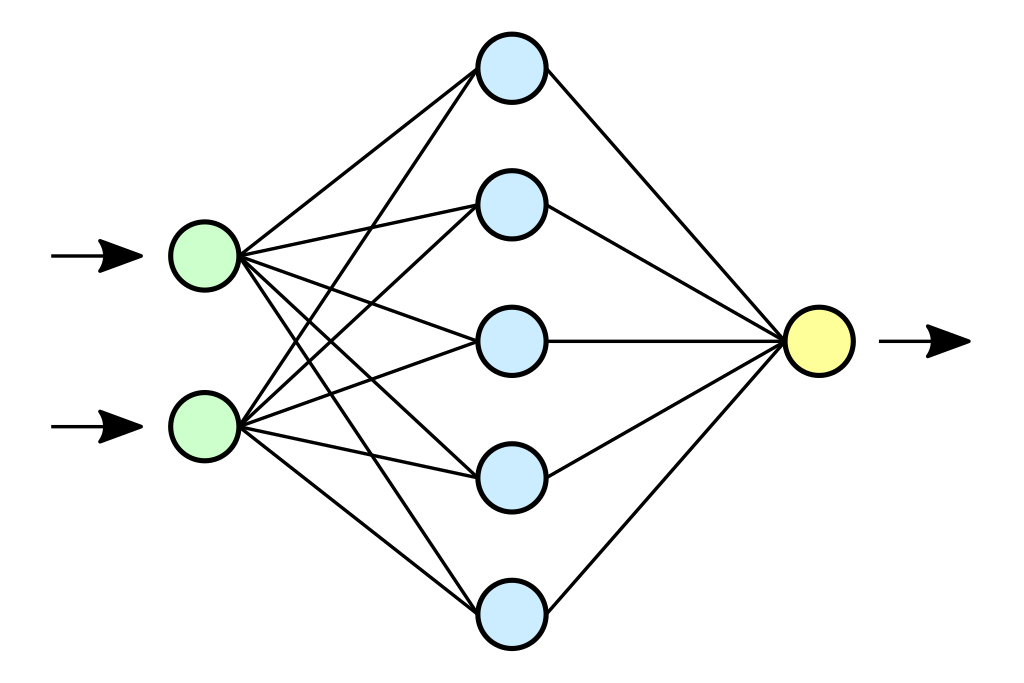
\includegraphics[width=\linewidth]{assets/simple_neural_network.png}\\
%         Neural Network
%     \end{minipage}\hfill
%     %
%     \note{And at the end we have an output distribution of the predicted classes}
%     \begin{minipage}{0.2\linewidth}
%         \centering
%         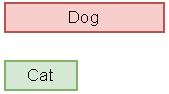
\includegraphics[width=\linewidth]{assets/wrong_y_prob.pdf}\\
%         Output Distribution
%     \end{minipage}    
% \end{frame}

% \begin{frame}{Neural Network Training}
%     At the end of the day, we have:
%     \vfill
%     \begin{enumerate}
%         \item Neural network classifier (parametrized)
%         \item Input data (labeled)
%         \item \highlight{Loss function to optimize}
%     \end{enumerate}
% \end{frame}

% \begin{frame}{Neural Network Training}
%     When the prediction is \highlight{wrong}:
%     \vfill

% \texttransparent{0.35}{
%     \begin{minipage}{0.2\linewidth}
%         \centering
%         
\includegraphics[width=\linewidth]{assets/input_cat.png}\\
%         Input image
%     \end{minipage}\hfill
% }
%     %
%     \begin{minipage}{0.4\linewidth}
%         \centering
%         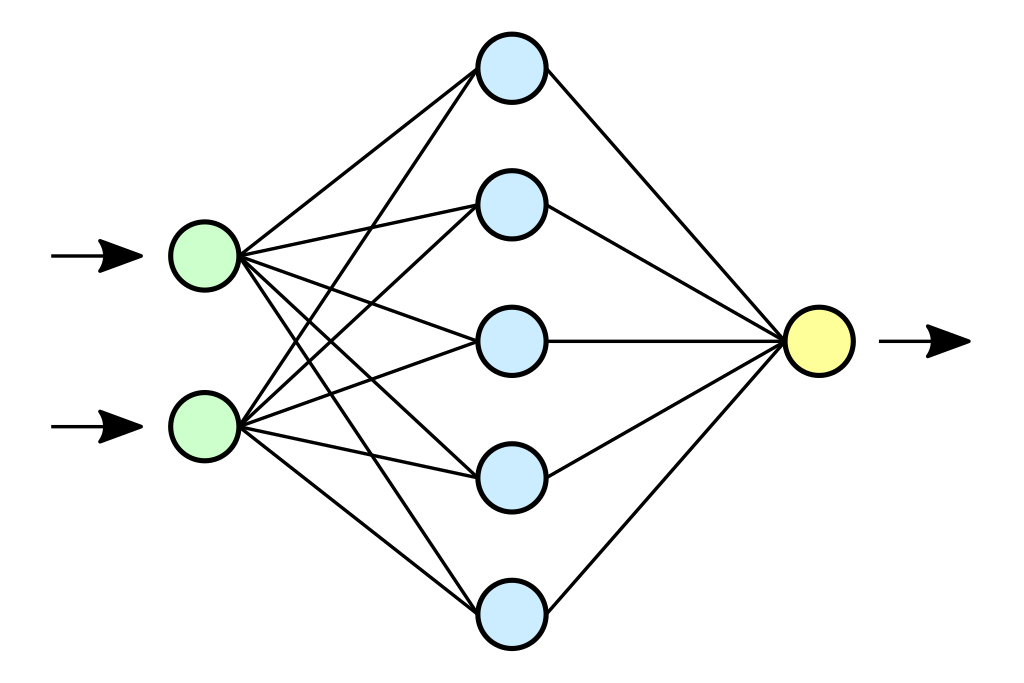
\includegraphics[width=\linewidth]{assets/simple_neural_network.png}\\
%         Neural Network
%     \end{minipage}\hfill
%     %
%     \begin{minipage}{0.2\linewidth}
%         \centering
%         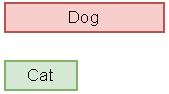
\includegraphics[width=\linewidth]{assets/wrong_y_prob.pdf}\\
%         Output Distribution
%     \end{minipage}    
% \end{frame}

% \begin{frame}{Neural Network Training}
%     When the prediction is wrong, we update the \highlight{model parameters},    according to $\nabla_\bW \loss$
%     \vfill

% \texttransparent{0.35}{
%     \begin{minipage}{0.2\linewidth}
%         \centering
%         
\includegraphics[width=\linewidth]{assets/input_cat.png}\\
%         Input image
%     \end{minipage}\hfill
% }
%     %
%     \begin{minipage}{0.4\linewidth}
%         \centering
%         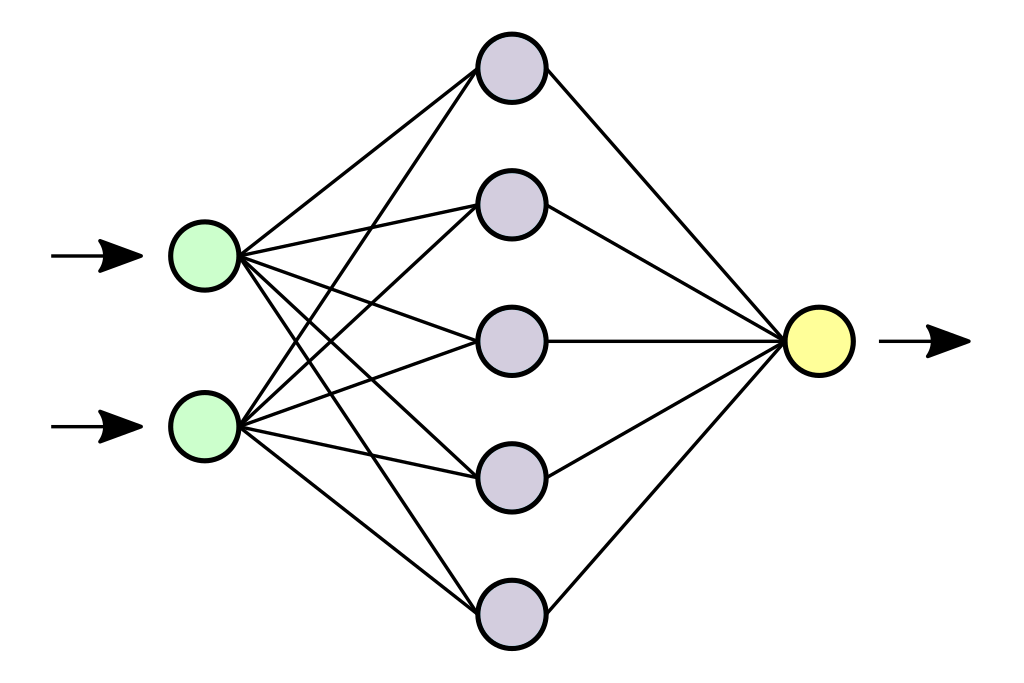
\includegraphics[width=\linewidth]{assets/simple_neural_network_2.png}\\
%         Neural Network
%     \end{minipage}\hfill
%     %
%     \begin{minipage}{0.2\linewidth}
%         \centering
%         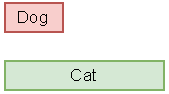
\includegraphics[width=\linewidth]{assets/correct_y_prob.pdf}\\
%         Output Distribution
%     \end{minipage}    
% \end{frame}


\begin{frame}{Gradient-based Attacks}
\note{
    When training a neural network in a supervised setting, we have some input, some randomly initialized weights and a ground-truth.\\
    But when doing a gradient-based attack, we aim to make a neural network misclassify a given input.\\
    To do that, we have to optimize the input instead, according to the Loss function.\\
}

    We want to \highlight{change the input} to minimize the loss\\
    \vfill

    \begin{minipage}{0.2\linewidth}
        \centering
        
\includegraphics[width=\linewidth]{assets/input_cat.png}\\
        Input image
    \end{minipage}\hfill
    %
    \begin{minipage}{0.4\linewidth}
        \centering
        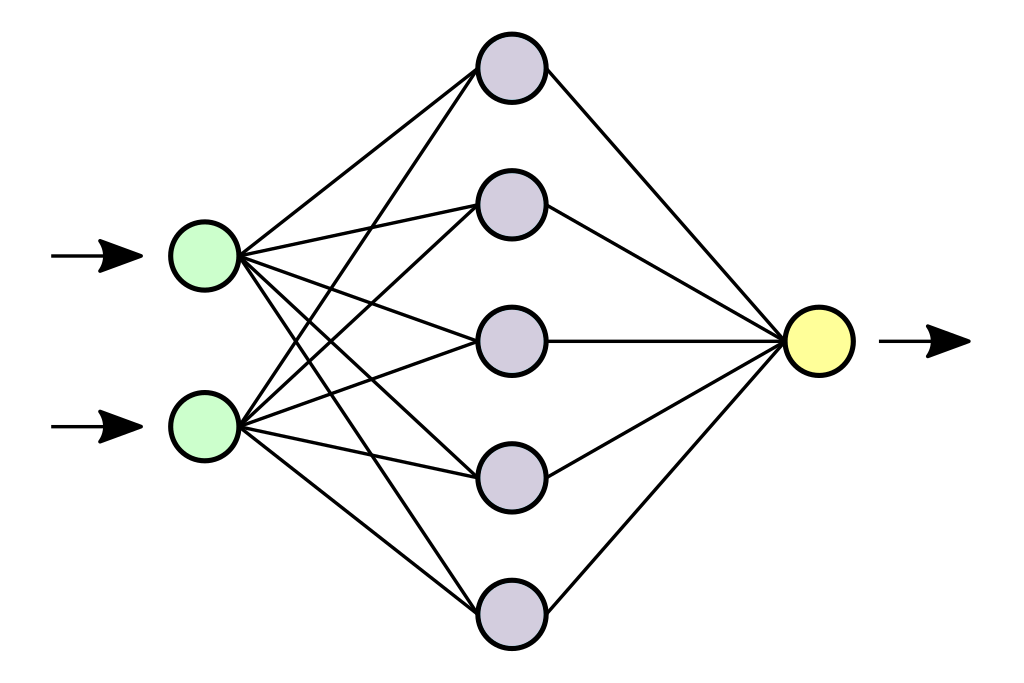
\includegraphics[width=\linewidth]{assets/simple_neural_network_2.png}\\
        Neural Network
    \end{minipage}\hfill
    %
    \begin{minipage}{0.2\linewidth}
        \centering
        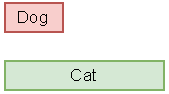
\includegraphics[width=\linewidth]{assets/correct_y_prob.pdf}\\
        Output Distribution
    \end{minipage}    
\end{frame}

% \begin{frame}{Gradient-based Attacks}
%     What to optimize?
%     \vfill

%     \begin{minipage}{0.2\linewidth}
%         \centering
%         
\includegraphics[width=\linewidth]{assets/input_cat.png}\\
%         Input image
%     \end{minipage}\hfill
%     + $\alpha \cdot$\hfill
%     %
%     \begin{minipage}{0.2\linewidth}
%         \centering
%         
\includegraphics[width=\linewidth]{assets/noise.png}\\
%         Noise
%     \end{minipage}\hfill
%     $\Rightarrow$\hfill
%     %
%     \begin{minipage}{0.2\linewidth}
%         \centering
%         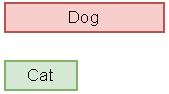
\includegraphics[width=\linewidth]{assets/wrong_y_prob.pdf}\\
%         Output Distribution
%     \end{minipage}
% \end{frame}


\begin{frame}{Gradient-based Attacks}
\note{
    However, we do not directly optimize the input image, but a delta noise, weighted by an alpha factor.\\
    This way, the input is the sum of the two, and hopefully, the model will misclassify.\\
}
    What to optimize?
    \vfill

    \begin{minipage}{0.2\linewidth}
        \centering
        
\includegraphics[width=\linewidth]{assets/input_cat.png}\\
        Input image
    \end{minipage}\hfill
    + $\alpha \cdot$\hfill
    %
    \begin{minipage}{0.2\linewidth}
        \centering
        
\includegraphics[width=\linewidth]{assets/noise.png}\\
        \highlight{Noise}
    \end{minipage}\hfill
    %
    $\Rightarrow$\hfill
    %
    \begin{minipage}{0.2\linewidth}
        \centering
        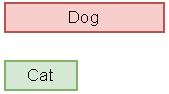
\includegraphics[width=\linewidth]{assets/wrong_y_prob.pdf}\\
        Output Distribution
    \end{minipage}
\end{frame}

% \begin{frame}{Example of Targeted Attack}
%     Given fixed:
%     \begin{itemize}
%         \item Input sample $\bx$
%         \item Frozen classifier $C$
%         \item Target class $t$ to be wrongly predicted
%     \end{itemize}

%     \begin{equation*}
%         \min_{\delta \in [0,1]^n} \alpha \; || \delta || + \loss_\text{CE}(f_\theta(\bx + \delta), t)
%     \end{equation*}

%     \vfill
%     \footnotesize
%     \centering
%     Carlini and Wagner, “Towards Evaluating the Robustness of Neural Networks”, 2016
% \end{frame}

% \begin{frame}{Untargeted Attacks}
%     Given fixed:
%     \begin{itemize}
%         \item Input sample $\bx$
%         \item Frozen classifier $C$
%     \end{itemize}

%     \begin{equation*}
%         \bx' = \bx \;\text{\highlight{+}}\; \alpha \cdot \text{sign}(\nabla_\bx \loss(\bx, y))
%     \end{equation*}

%     \begin{center}
%     This time, we are \highlight{maximizing} the loss function,\\
%     to make the classifier go in the \emph{opposite} direction of being right
%     \end{center}

%     \vfill
%     \footnotesize
%     \centering
%     Kurakin et al, “Adversarial examples in the physical world”, 2016
% \end{frame}

\begin{frame}{Adversarial Input}
\note{
    At the end of this optimization process, the adversarial image may look like this: \\
    it does not look different to a human eye, but it is sufficiently different to fool a deep classifier.
}
    The optimized perturbation $\delta$ may look like:
    \vfill

    \begin{minipage}{0.2\linewidth}
        \centering
        
\includegraphics[width=\linewidth]{assets/input_cat.png}\\
        Input image
    \end{minipage}\hfill
    + $\alpha \cdot$\hfill
    %
    \begin{minipage}{0.2\linewidth}
        \centering
        
\includegraphics[width=\linewidth]{assets/noise.png}\\
        Noise
    \end{minipage}\hfill
    $\Rightarrow$\hfill
    %
    \begin{minipage}{0.2\linewidth}
        \centering
        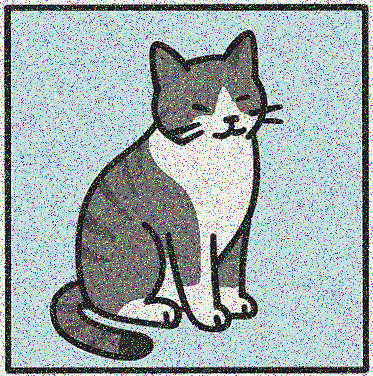
\includegraphics[width=\linewidth]{assets/input_cat_noise.png}\\
        \highlight{Adversarial image}
    \end{minipage}
\end{frame}

% \begin{frame}{Wrong Prediction}
%     We made our first adversarial attack!
%     \vfill

%     \begin{minipage}{0.2\linewidth}
%         \centering
%         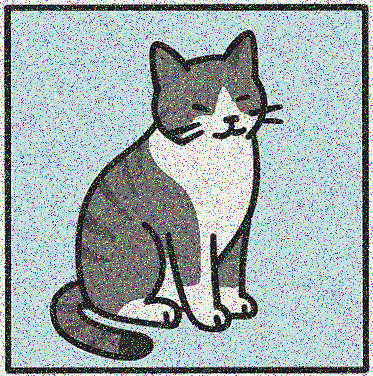
\includegraphics[width=\linewidth]{assets/input_cat_noise.png}\\
%         Adversarial input image
%     \end{minipage}\hfill
%     $\Rightarrow$\hfill
%     %
%     \begin{minipage}{0.4\linewidth}
%         \centering
%         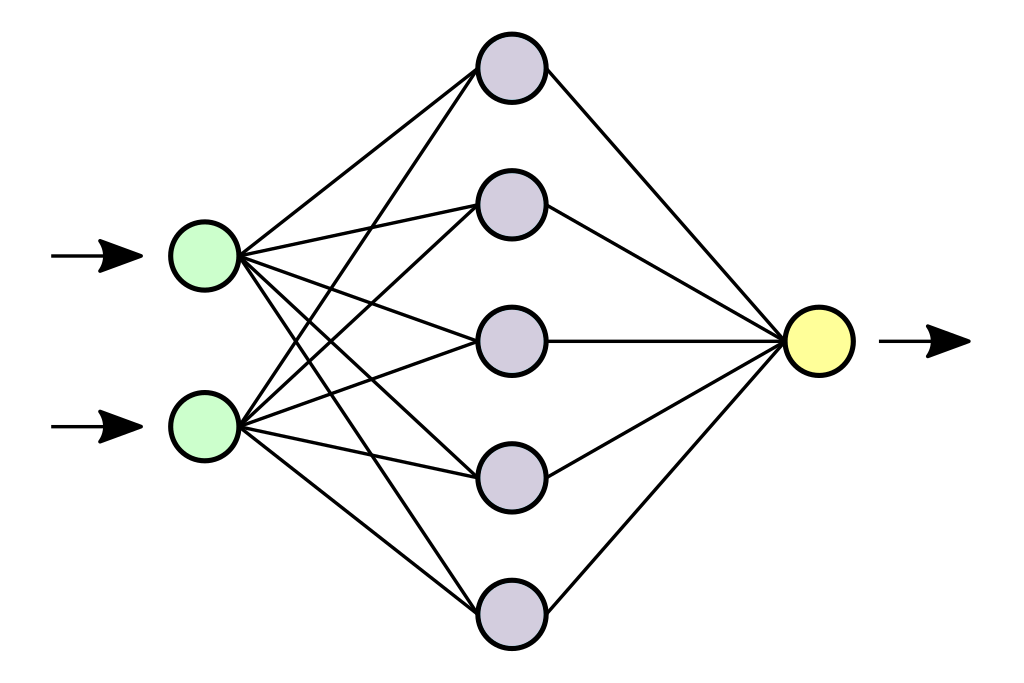
\includegraphics[width=\linewidth]{assets/simple_neural_network_2.png}\\
%         Unchanged neural network
%     \end{minipage}\hfill
%     $\Rightarrow$\hfill
%     %
%     \begin{minipage}{0.2\linewidth}
%         \centering
%         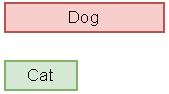
\includegraphics[width=\linewidth]{assets/wrong_y_prob.pdf}\\
%         Wrong prediction
%     \end{minipage}
% \end{frame}

% \begin{frame}{Not a Robust Classifier}
%     As humans we still see a cat, not a dog, in the adversarial image.\\
%     This classifier is \highlight{not} robust!
%     \vfill

%     \begin{figure}
%         \centering
%         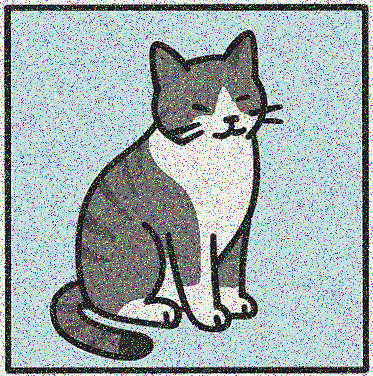
\includegraphics[width=0.2\linewidth]{assets/input_cat_noise.png}
%         \caption{Not a dog}
%     \end{figure}
% \end{frame}


\begin{frame}{Adversarial Training}
\note{
    Here it comes Adversarial Training. \\
    It is a procedure that generally proceeds as follows: \\
    - we generate adversarial samples in some way, for instance as just said \\
    - they are included in the training process to let the model know their correct class and make it classify them correctly \\
    - and we iterate. \\
    --------- PAUSE --------- \\
    Then, what happens? \\
    The required perturbation may be always more and more visible to human eyes.
}
    A classifier can be made robust using \highlight{Adversarial Training}:
    \begin{itemize}
        \item Generate $\bx'$ samples
        \item Include them in the training process
        \item Repeat
    \end{itemize}
    
    \pause
    \vfill
    The required perturbation $\delta$ will be more and more perceptible by humans
    \vspace{0.5cm}

    \begin{minipage}{0.15\textwidth}
        
\includegraphics[width=\textwidth]{assets/input_cat.png}
    \end{minipage}
    \hfill
    \begin{minipage}{0.15\textwidth}
        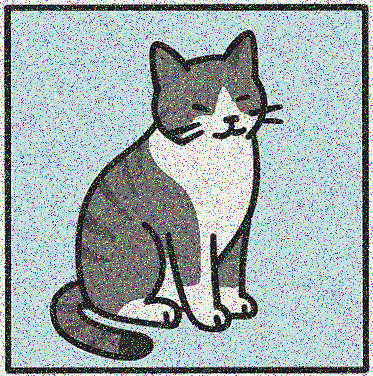
\includegraphics[width=\textwidth]{assets/input_cat_noise.png}
    \end{minipage}
    \hfill
    \begin{minipage}{0.15\textwidth}
        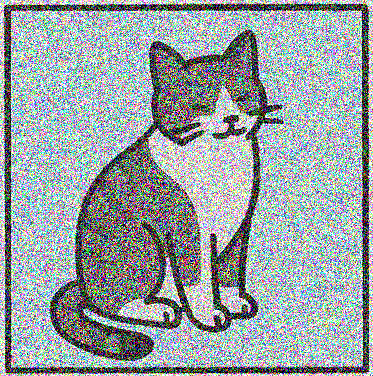
\includegraphics[width=\textwidth]{assets/input_cat_noise_strong.png}
    \end{minipage}
\end{frame}

% \begin{frame}{Perceptually-Aligned Gradients}
%     \centering
%     The required perturbation $\delta$ will be \highlight{more and more perceptible} by humans \\
%     until we get to \highlight{PAG}
% \end{frame}

\begin{frame}{Perceptually-Aligned Gradients}
\note{
    Until something interesting has been observed in literature to happen: \\
    gradients start to make sense! \\
    These are examples of perturbations that we have to apply to our small bird to be misclassified. \\
    They can be perceived by humans as THE OTHER CLASS! \\
    That's why it has this name: Perceptually-Aligned Gradients. \\
    --------- \\
    The best point is that researchers discovered that enforcing PAG on a model in the training procedure makes it Robust. \\
    Can we do the same on LLMs?
}
    When our classifier has PAGs:

    \begin{figure}
        \begin{minipage}{0.25\textwidth}
            \centering
            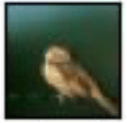
\includegraphics[width=0.8\textwidth]{assets/pag_original_bird.png}
            \caption{Original image: bird}
        \end{minipage}\hfill
        \begin{minipage}{0.25\textwidth}
            \centering
            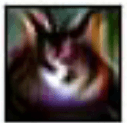
\includegraphics[width=0.8\textwidth]{assets/pag_attack_cat.png}
            \caption{A "bird" classified as cat}
        \end{minipage}\hfill
        \begin{minipage}{0.25\textwidth}
            \centering
            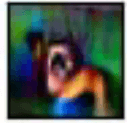
\includegraphics[width=0.8\textwidth]{assets/pag_attack_dog.png}
            \caption{A "bird" classified as dog}
        \end{minipage}
    \end{figure}

    \vfill
    \centering
    \textbf{Gradients are aligned to the} \highlight{human perception}

    \vspace{0.3cm}
    \footnotesize
    \centering
    Ganz et al, "Do Perceptually Aligned Gradients Imply Robustness?", 2023
\end{frame}

% \begin{frame}{Enforcing PAG}
%     The loss function becomes more complex:

%     \begin{equation*}
%         \mathcal{L}(x, y) = \mathcal{L}_{CE}( f_\theta(x), y)
%                 \textcolor{navy}{%
%                 + \lambda \frac{1}{C} \sum_{y_t=1}^C \mathcal{L}_{cos}(\nabla_x f_\theta(x)_{y_t}, g(x, y_t))%
%                 }
%     \end{equation*}
% \end{frame}

% \begin{frame}{PAG Loss}
%     Not that complex

%     \begin{equation*}
%         \frac{1}{C} \sum_{y_t=1}^C
%         \pause\mathcal{L}_{cos}(
%         \pause\nabla_x f_\theta(x)_{y_t},
%         \pause g(x, y_t))
%     \end{equation*}

%     \begin{figure}
%         \centering
%         \includegraphics[width=0.45\linewidth]{assets/pag_point_cloud.png}
%     \end{figure}
% \end{frame}

% \begin{frame}{Defining g()}
%     It is the ground truth of the gradients on $\bx$ that a robust classifier should have.

%     We do not have them, since we do not have a robust classifier yet.

%     \pause\vfill
%     \note{
%     There are multiple ways to define it.
%     \\
%     To keep things simple, use the difference between the current sample $x$ and a random sample $u_y$, different from $x$, of class $y$
%     }

%     A simple possible formulation:
%     \begin{equation*}
%         g(x, y) = u_y - x \quad\text{s.t.}\; u_y \in C_y \;\wedge\; u_y \neq x
%     \end{equation*}

%     \pause\vfill
%     \textbf{Note:} the $y$ argument of $g(x, y)$ can be \textbf{any} class, not only the real class of $x$
% \end{frame}


